\documentclass[11pt]{article}
\usepackage[margin=1in]{geometry}
\usepackage{booktabs}
\usepackage{amsmath}
\usepackage{graphicx}
\usepackage{hyperref}
\hypersetup{colorlinks=true, linkcolor=blue, urlcolor=blue}
\sloppy

% Every number in this document --- prose included --- is defined by
% acquire_external_data.py in these two generated files. Nothing is typed by hand.
% GENERATED BY acquire_external_data.py — do not edit by hand.
% Every number that appears in the memo's prose is defined here.
\newcommand{\acqAsrBalanced}{4{,}372}
\newcommand{\acqAsrFirst}{2007}
\newcommand{\acqAsrFound}{5{,}565}
\newcommand{\acqAsrGapYears}{9}
\newcommand{\acqAsrJoin}{81.6}
\newcommand{\acqAsrLast}{2025}
\newcommand{\acqAsrNYears}{19}
\newcommand{\acqAsrParcels}{222{,}251}
\newcommand{\acqAsrParcelsPerYear}{208{,}927}
\newcommand{\acqAsrRows}{3{,}934{,}467}
\newcommand{\acqAsrSought}{8{,}294}
\newcommand{\acqBridgeCU}{46.0}
\newcommand{\acqBridgeCUN}{2{,}336}
\newcommand{\acqBridgeCUTotal}{5{,}074}
\newcommand{\acqBridgeDR}{71.8}
\newcommand{\acqBridgeDbi}{7{,}833}
\newcommand{\acqBridgeDbiShare}{48.4}
\newcommand{\acqBridgeDnt}{57.3}
\newcommand{\acqBridgeItems}{7{,}875}
\newcommand{\acqBridgeLpa}{70.5}
\newcommand{\acqBridgePca}{7.6}
\newcommand{\acqBridgeShare}{48.6}
\newcommand{\acqBridgeVar}{63.3}
\newcommand{\acqCaseAny}{92.7}
\newcommand{\acqCaseAnyN}{8{,}334}
\newcommand{\acqCaseJoinBreakYear}{2002}
\newcommand{\acqCaseJoinLateMin}{96}
\newcommand{\acqCaseNorm}{75.0}
\newcommand{\acqCaseRaw}{74.7}
\newcommand{\acqCaseStem}{92.7}
\newcommand{\acqCases}{8{,}987}
\newcommand{\acqClDenseFirst}{1968}
\newcommand{\acqClFirst}{1900}
\newcommand{\acqClItemKeys}{8{,}294}
\newcommand{\acqClItemKeysTraded}{3{,}882}
\newcommand{\acqClItemKeysTradedPct}{46.8}
\newcommand{\acqClItemsEver}{7{,}727}
\newcommand{\acqClItemsEverPct}{56.7}
\newcommand{\acqClItemsNear}{3{,}125}
\newcommand{\acqClItemsNearPct}{22.9}
\newcommand{\acqClKeyed}{100.0}
\newcommand{\acqClLast}{2024}
\newcommand{\acqClMaxDate}{2024-05-16}
\newcommand{\acqClMedianRecent}{1.42}
\newcommand{\acqClParcels}{174{,}102}
\newcommand{\acqClPriced}{415{,}854}
\newcommand{\acqClResidential}{320{,}323}
\newcommand{\acqClRows}{447{,}883}
\newcommand{\acqClWindowYears}{3}
\newcommand{\acqCoreLogicSales}{415{,}854}
\newcommand{\acqCorpusSpan}{1998--2026}
\newcommand{\acqCuHousingProd}{17.6}
\newcommand{\acqCuMohcd}{1.5}
\newcommand{\acqCuPipeline}{4.5}
\newcommand{\acqCuUnits}{91.9}
\newcommand{\acqCuUnitsNZ}{27.1}
\newcommand{\acqCuUnitsNZearly}{18.3}
\newcommand{\acqCuUnitsNZlate}{30.9}
\newcommand{\acqDelayIssueMedian}{245}
\newcommand{\acqDelayIssuePninety}{768}
\newcommand{\acqDemandFiles}{76}
\newcommand{\acqDemandGB}{4.92}
\newcommand{\acqDistinctParcelKeys}{8{,}294}
\newcommand{\acqEitherCU}{46.1}
\newcommand{\acqEitherDR}{93.2}
\newcommand{\acqEitherRoute}{54.0}
\newcommand{\acqFeeAreaRows}{33}
\newcommand{\acqFeeEarliestSnapshot}{2019-09-15}
\newcommand{\acqFeeFirst}{2019}
\newcommand{\acqFeeLast}{2026}
\newcommand{\acqFeeRates}{1{,}341}
\newcommand{\acqFeeRegisters}{8}
\newcommand{\acqInclusionaryFirst}{199.50}
\newcommand{\acqInclusionaryLast}{249.66}
\newcommand{\acqItems}{16{,}199}
\newcommand{\acqLagCU}{175}
\newcommand{\acqLagCoverage}{92.7}
\newcommand{\acqLagDR}{105}
\newcommand{\acqLagMedian}{142}
\newcommand{\acqLagN}{8{,}334}
\newcommand{\acqLagNegative}{0.3}
\newcommand{\acqLagPninety}{758}
\newcommand{\acqLagPninetynine}{2346}
\newcommand{\acqLagTrunc}{1{,}500}
\newcommand{\acqLagVar}{280}
\newcommand{\acqLandUseMulti}{77}
\newcommand{\acqMinCasesFig}{10}
\newcommand{\acqMinItemsBridge}{100}
\newcommand{\acqModernUnmatched}{92}
\newcommand{\acqMohcdMaxYear}{2030}
\newcommand{\acqMohcdRows}{190}
\newcommand{\acqNonProjRows}{233{,}394}
\newcommand{\acqNonUniqueSources}{14}
\newcommand{\acqNpApplicant}{66.9}
\newcommand{\acqNpApplicantOrg}{34.3}
\newcommand{\acqNpBuildingPermits}{22.9}
\newcommand{\acqNpCloseDate}{94.9}
\newcommand{\acqNpMinYear}{1920}
\newcommand{\acqNpOpenDate}{100.0}
\newcommand{\acqNpParentId}{26.7}
\newcommand{\acqNpPlanner}{77.7}
\newcommand{\acqNpRecordStatus}{100.0}
\newcommand{\acqOldFormatCases}{536}
\newcommand{\acqOldFormatMatched}{0}
\newcommand{\acqParcelActive}{66.9}
\newcommand{\acqParcelJoin}{89.5}
\newcommand{\acqParcelJoinN}{12{,}195}
\newcommand{\acqParcelNoBlock}{193}
\newcommand{\acqParcelNoLot}{1{,}232}
\newcommand{\acqParcelRetired}{3{,}080}
\newcommand{\acqParcelRows}{236{,}556}
\newcommand{\acqParcelShare}{84.1}
\newcommand{\acqPipelineRows}{1{,}917}
\newcommand{\acqPrBuildingPermits}{45.2}
\newcommand{\acqPrDecision}{18.3}
\newcommand{\acqPrDecisionDate}{17.3}
\newcommand{\acqPrEnvDoc}{25.1}
\newcommand{\acqPrInclFlag}{2.9}
\newcommand{\acqPrUnitsAff}{100.0}
\newcommand{\acqPrUnitsNet}{94.0}
\newcommand{\acqPrUnitsProp}{100.0}
\newcommand{\acqPrintedAll}{22.1}
\newcommand{\acqPrintedCU}{0.3}
\newcommand{\acqPrintedDR}{85.5}
\newcommand{\acqProjRows}{54{,}515}
\newcommand{\acqRetrieved}{2026-09-08}
\newcommand{\acqScaleEarliest}{2005}
\newcommand{\acqSourcesCached}{19}
\newcommand{\acqTsfNinetyNineFirst}{10.29}
\newcommand{\acqTsfNinetyNineLast}{13.39}
\newcommand{\acqUcMaxYear}{2205}
\newcommand{\acqWithParcel}{13{,}620}
\newcommand{\acqZhviFirst}{2000-01}
\newcommand{\acqZhviLast}{2026-07}
\newcommand{\acqZhviMonths}{319}
\newcommand{\acqZhviZips}{26}
\newcommand{\acqZoningParcelSpan}{1998--2008}
\newcommand{\acqZoningParcelYears}{9}
\newcommand{\acqZoningPolygonYears}{11}
\newcommand{\acqZoriFirst}{2015-01}
\newcommand{\acqZoriLast}{2026-07}
\newcommand{\acqZoriMonths}{139}
\newcommand{\acqZoriZips}{24}


\title{Locating the Next Tranche:\\
\large A denominator, a clock, a scale, a price and a fee schedule for the
item panel}
\author{Dan Post}
\date{September 2026}

\begin{document}
\maketitle

\begin{abstract}
\noindent
The paper is moving to a real-options frame, and that changes what the data has to do. The
outcome of interest becomes the \emph{filing} decision, which needs a denominator --- the
parcels that could have produced a case and did not --- and the developer's clock starts at
filing, not at the first hearing. The item table is a numerator measured from the wrong
instant. This memo finds, verifies, caches and measures the five categories of data that fix
that, and records the negatives so nobody runs these searches again.

\medskip\noindent
Five results.

\medskip\noindent
\textbf{First, the parcel risk set exists and the panel is shorter than the corpus.} DataSF's
parcel layer holds \acqParcelRows\ parcels, active and retired, on a unique
\texttt{blklot} key, and \acqParcelJoinN\ of the \acqWithParcel\ items that carry a parcel
key --- \acqParcelJoin\% --- join to it. That is below the 95\% the brief asked for, and the
shortfall is not formatting: \acqParcelNoLot\ items name a block that exists and a lot that
never did. The value side is the assessor's secured roll (\texttt{wv5m-vpq2}, the proposed
identifier, verified): \acqAsrRows\ parcel-years over \acqAsrParcels\ parcels --- but roll
years \acqAsrFirst--\acqAsrLast, not \acqCorpusSpan. \textbf{\acqAsrGapYears\ years of the
corpus have no assessed value at all}, and that is the binding constraint on the risk set, not a scrape
artefact. Zoning is better than expected: \acqZoningParcelYears\ vintages,
\acqZoningParcelSpan, are
published \emph{parcel-keyed} and join directly; \acqZoningPolygonYears\ more are polygons.

\medskip\noindent
\textbf{Second, the case number joins the Planning Department's records at \acqCaseAny\%},
and that buys the pre-hearing wait. Raw string equality reaches only \acqCaseRaw\%; stripping
the case-number suffix reaches \acqCaseStem\%. For the \acqLagN\ cases that join,
\textbf{the median wait from filing to first hearing is \acqLagMedian\ days}, the 90th
percentile \acqLagPninety\ and the 99th \acqLagPninetynine. The delay memo reports a
\acqDelayIssueMedian-day median from hearing to permit issuance, with a 90th percentile of
\acqDelayIssuePninety, and has nothing before the hearing. The wait it could not see has a
smaller median and essentially the same 90th percentile --- so, relative to its own centre, it
is the more dispersed of the two, which is exactly the quantity a real-options threshold
responds to.

\medskip\noindent
\textbf{Third --- the most consequential finding --- the \texttt{building\_permits} bridge
works, and it overturns the conditions memo.} That memo (\S5.1) concludes that the permit
route reaches discretionary review and the conditions route reaches conditional use, and that
``they never cover the same item.'' Following a conditional use through its planning record to
the permit numbers the department itself attaches, \textbf{\acqBridgeCUN\ of \acqBridgeCUTotal\
conditional-use items --- \acqBridgeCU\% --- reach a permit that is present in DBI},
against the \acqPrintedCU\% that print one in the minutes. The non-overlap is not a property
of the world; it was a property of the one route we had. Across the whole docket
\acqEitherRoute\% of items now reach a real building permit by some route.

\medskip\noindent
\textbf{Fourth, project scale is reachable but thin where it matters.} A unit count is
attached to \acqCuUnits\% of conditional-use items through the Projects table --- and is
\emph{non-zero} on \acqCuUnitsNZ\%. The purpose-built pipeline datasets are worse: the
Development Pipeline reaches \acqCuPipeline\% and is a current snapshot, and Housing
Production reaches \acqCuHousingProd\% by parcel.

\medskip\noindent
\textbf{Fifth, the price side is stronger than expected, and it joins on the parcel key.} The
CoreLogic/Cotality extract is on disk under the data root: \textbf{\acqClPriced\
arms-length priced San Francisco sales, \acqClDenseFirst--\acqClLast, over \acqClParcels\
parcels}. Cotality prints San Francisco's APN as block and lot, so it is not a block-group
price --- it is \texttt{blklot}, the same key as \S2, on \acqClKeyed\% of transactions.
\textbf{\acqClItemsEverPct\% of items carrying a parcel key sit on a parcel that has
traded}, and \acqClItemsNearPct\% on one that traded within \acqClWindowYears\ years of
the hearing itself. Zillow and the assessor's values are cached behind it as fallbacks. On
fees, \acqFeeRegisters\ annual
Citywide Development Impact Fee Registers, \acqFeeFirst--\acqFeeLast, parsed to
\acqFeeRates\ dated rate observations keyed by Planning Code section --- the Transportation
Sustainability Fee for residential projects over 99 units runs \$\acqTsfNinetyNineFirst\ to
\$\acqTsfNinetyNineLast\ per gross square foot over those \acqFeeRegisters\ years, and the
inclusionary
fee \$\acqInclusionaryFirst\ to \$\acqInclusionaryLast\ per square foot.
\end{abstract}

\tableofcontents
\newpage

\section{What this memo is for, and what ``found'' means in it}

A developer sinks entitlement cost before the hearing outcome resolves. Dispersion in delay
and in conditions raises the rent threshold at which filing is worth doing at all, so the
observable consequence of a demanding Commission is not worse projects but \emph{fewer and
higher-value} ones. Two things follow for the data, and everything below serves one of them.

\begin{enumerate}
\item The outcome is the \textbf{filing decision}, so the analysis needs a population at
risk. The item table is a numerator: it holds the requests that were made. The denominator is
every parcel in the city that could have produced a request and did not.
\item The developer's clock starts at \textbf{filing}. Every delay measure in the pipeline
today starts at the first hearing, which is well downstream of the decision being modelled.
\end{enumerate}

\paragraph{Found, usable, and the difference.} This memo reports a source as \emph{usable}
only when the join key is present \emph{and} the join rate has been measured against the item
table. A file that downloaded is not a result. Where a dataset's documentation promises a
field and the rows are empty, the empty rate is reported and not the documentation ---
Table~\ref{tab:recordfields} is that table, and \S\ref{sec:scale} contains the sharpest
instance of it.

\paragraph{Two identifier facts that will bite anyone reusing this.} Both were found by the
probe stage and neither could have been assumed.

\begin{itemize}
\item \textbf{DataSF's Socrata domain is now \texttt{data.sf.gov}.} The old
\texttt{data.sfgov.org} still answers the \emph{resource} endpoint --- which is why
\texttt{analyze\_permits.py} keeps working --- but the \emph{catalogue} API indexes only the
new domain. A catalogue search against the old host returns zero hits and looks exactly like
``the dataset does not exist.'' Every dataset in this memo was resolved against the live
catalogue on \acqRetrieved\ and the identifier reported in Table~\ref{tab:inventory} is the
one actually used.
\item \textbf{\texttt{wv5m-vpq2} is the right assessor identifier} --- the brief's proposed
ID, verified --- \textbf{but the roll starts at \acqAsrFirst}. That is not a gap in a scrape; no
earlier vintage is published. It is reported as a negative in
Table~\ref{tab:negatives} because the temptation to go looking again will be strong.
\item \textbf{A Dropbox subtree that has never been materialised is invisible to
\texttt{ls} and \texttt{find}.} The macOS file provider holds files online-only: the
directory entry carries the full size while the file occupies no blocks, and an
un-materialised directory does not list at all. The first pass of this memo concluded on that
basis that the CoreLogic extract was gone. It was not --- it was dehydrated, and \S5 is what
it actually contains. \texttt{acquire\_external\_data.py sync} now reports nominal bytes
against bytes on disk, which is the only way to tell the two cases apart.
\end{itemize}

% GENERATED BY acquire_external_data.py — do not edit by hand.
\begin{table}[htbp]\centering
\caption{Every identifier resolved against the live catalogue on 2026-09-08. `Key unique' is tested on the cached rows, not assumed: DBI's \texttt{permit\_number} was not unique and 145{,}795 rows repeated one. A dash means the column is not a key we join on.}\label{tab:inventory}
\resizebox{\textwidth}{!}{%
\begin{tabular}{llrrll}\toprule
Dataset & Identifier & Rows & Distinct key & Key unique & Date range\\\midrule
\multicolumn{6}{l}{\emph{Fees}}\\
\quad Neighborhood-Specific Impact Fee Areas & \texttt{ntc3-dd64} & 33 & 33 & yes & ---\\
\multicolumn{6}{l}{\emph{Filing dates}}\\
\quad Planning Department Records --- Non-Projects & \texttt{y673-d69b} & 233{,}394 & 233{,}394 & yes & 1920-04-07--2026-09-04\\
\quad Planning Department Records --- Projects & \texttt{qvu5-m3a2} & 54{,}515 & 54{,}515 & yes & 1974-05-21--2026-09-04\\
\multicolumn{6}{l}{\emph{Parcel risk set}}\\
\quad Assessor Historical Secured Property Tax Rolls & \texttt{wv5m-vpq2} & 3{,}934{,}467 & 222{,}251 & no (3{,}712{,}216 repeats) & 2007--2025\\
\quad Parcels --- Active and Retired & \texttt{acdm-wktn} & 236{,}556 & 236{,}556 & yes & 1984-07-31--2026-09-02\\
\quad San Francisco Land Use & \texttt{c5ge-t6pj} & 153{,}765 & 153{,}754 & no (11 repeats) & 2026-08-17--2026-08-17\\
\multicolumn{6}{l}{\emph{Project scale}}\\
\quad Dwelling Unit Completion Counts by Building Permit & \texttt{j67f-aayr} & 2{,}541 & 2{,}420 & no (121 repeats) & 2002-04-01--2205-03-13\,\emph{(sic)}\\
\quad Housing Production --- 2005--present & \texttt{xdht-4php} & 6{,}139 & 5{,}146 & no (993 repeats) & 2005-01-03--2026-08-28\\
\quad MOHCD Affordable Housing Pipeline & \texttt{aaxw-2cb8} & 190 & 131 & no (59 repeats) & 1995-09-19--2030-03-15\\
\quad San Francisco Development Pipeline & \texttt{6jgi-cpb4} & 1{,}917 & 1{,}793 & no (124 repeats) & 1997-06-12--2026-07-28\\
\multicolumn{6}{l}{\emph{Zoning (parcel-keyed)}}\\
\quad Historic Zoning Districts --- 1998 & \texttt{piqy-pimd} & 152{,}569 & 152{,}535 & no (34 repeats) & ---\\
\quad Historic Zoning Districts --- 2000 & \texttt{itx2-wzp5} & 153{,}292 & 153{,}247 & no (45 repeats) & ---\\
\quad Historic Zoning Districts --- 2001 & \texttt{8m6w-8yuk} & 153{,}669 & 153{,}593 & no (76 repeats) & ---\\
\quad Historic Zoning Districts --- 2002 & \texttt{3yi7-eyfd} & 153{,}663 & 153{,}582 & no (81 repeats) & ---\\
\quad Historic Zoning Districts --- 2003 & \texttt{6ru7-zq4y} & 153{,}716 & 153{,}518 & no (198 repeats) & ---\\
\quad Historic Zoning Districts --- 2004 & \texttt{s3eh-jdwb} & 191{,}062 & 190{,}896 & no (166 repeats) & ---\\
\quad Historic Zoning Districts --- 2005 & \texttt{b52k-gy2v} & 196{,}344 & 192{,}031 & no (4{,}313 repeats) & ---\\
\quad Historic Zoning Districts --- 2007 & \texttt{pe87-v8tx} & 153{,}822 & 153{,}751 & no (71 repeats) & ---\\
\quad Historic Zoning Districts --- 2008 & \texttt{tsdh-z53a} & 153{,}355 & 153{,}355 & yes & ---\\
\bottomrule\end{tabular}}\end{table}

\begin{table}[htbp]\centering
\caption{The parcel join, and what the residual is. The item table's key is \texttt{assessor\_block} plus each entry of \texttt{lot\_number}, zero-padded to DataSF's 4+3 \texttt{blklot} form; an item joins if any of its lots does. Percentages are of the 13{,}620 items that carry a parcel key at all.}\label{tab:parceljoin}
\begin{tabular}{lrr}\toprule
Items & Count & Share\\\midrule
All items in the corpus & 16{,}199 & 100.0\%\\
\quad carrying a block and at least one lot & 13{,}620 & 84.1\%\\
\quad\quad joined to \texttt{blklot} in the parcel layer & 12{,}195 & 89.5\%\\
\quad\quad\quad \dots\ to a parcel still active & 9{,}115 & 66.9\%\\
\quad\quad\quad \dots\ to a retired parcel only & 3{,}080 & 22.6\%\\
\quad\quad joined to \texttt{mapblklot} (the surviving map parcel) & 12{,}038 & 88.4\%\\
\quad\quad not joined: block exists, that lot does not & 1{,}232 & 9.0\%\\
\quad\quad not joined: no such block & 193 & 1.4\%\\
\bottomrule\end{tabular}\end{table}

\begin{table}[htbp]\centering
\caption{The assessor roll as a parcel-year panel, and how far it reaches. The panel is unbalanced by construction --- a parcel enters when it is created and leaves when it is merged away --- and it starts at roll year 2007, which is the binding constraint on the risk set.}\label{tab:assessor}
\begin{tabular}{lr}\toprule
Quantity & Value\\\midrule
Rows (parcel-years) & 3{,}934{,}467\\
Distinct parcels & 222{,}251\\
Roll years & 2007--2025 (19 years)\\
Distinct item parcel keys sought & 8{,}294\\
\quad found on the roll & 5{,}565\\
\quad\quad median roll years observed for one of them & 19 of 19\\
\quad\quad present in every roll year & 4{,}372\\
Items with a parcel key joined to the roll & 11{,}112 (81.6\%)\\
\bottomrule\end{tabular}\end{table}

\begin{table}[htbp]\centering
\caption{Zoning, by how it is published. The parcel-keyed years join to the item table directly; the polygon years need a spatial join and are inventoried, not cached. 1999 is not published in either form.}\label{tab:zoning}
\resizebox{\textwidth}{!}{%
\begin{tabular}{llrrl}\toprule
Year & Identifier & Rows & Distinct \texttt{blklot} & Form\\\midrule
1998 & \texttt{piqy-pimd} & 152{,}569 & 152{,}535 & parcel-keyed (\texttt{blklot})\\
1999 & --- & 0 & --- & not published\\
2000 & \texttt{itx2-wzp5} & 153{,}292 & 153{,}247 & parcel-keyed (\texttt{blklot})\\
2001 & \texttt{8m6w-8yuk} & 153{,}669 & 153{,}593 & parcel-keyed (\texttt{mapblklot})\\
2002 & \texttt{3yi7-eyfd} & 153{,}663 & 153{,}582 & parcel-keyed (\texttt{blklot})\\
2003 & \texttt{6ru7-zq4y} & 153{,}716 & 153{,}518 & parcel-keyed (\texttt{blklot})\\
2004 & \texttt{s3eh-jdwb} & 191{,}062 & 190{,}896 & parcel-keyed (\texttt{blklot})\\
2005 & \texttt{b52k-gy2v} & 196{,}344 & 192{,}031 & parcel-keyed (\texttt{blklot})\\
2006 & \texttt{afkh-hfhr} & 23{,}132 & --- & polygon; needs a spatial join\\
2007 & \texttt{pe87-v8tx} & 153{,}822 & 153{,}751 & parcel-keyed (\texttt{blklot})\\
2008 & \texttt{tsdh-z53a} & 153{,}355 & 153{,}355 & parcel-keyed (\texttt{blklot})\\
2009 & \texttt{jud5-ja46} & 23{,}355 & --- & polygon; needs a spatial join\\
2010 & \texttt{x4gj-zjx7} & 9{,}897 & --- & polygon; needs a spatial join\\
2011 & \texttt{rt4q-mf68} & 9{,}880 & --- & polygon; needs a spatial join\\
2012 & \texttt{vfz8-awmy} & 9{,}889 & --- & polygon; needs a spatial join\\
2013 & \texttt{6jb9-g73z} & 9{,}982 & --- & polygon; needs a spatial join\\
2014 & \texttt{hg44-eza7} & 9{,}981 & --- & polygon; needs a spatial join\\
2015 & \texttt{ada2-cu6t} & 9{,}978 & --- & polygon; needs a spatial join\\
current (districts) & \texttt{xzez-p3nc} & 1{,}647 & --- & polygon; needs a spatial join\\
current (height and bulk) & \texttt{usp2-teig} & 1{,}195 & --- & polygon; needs a spatial join\\
current (special use) & \texttt{rxfc-8aap} & 125 & --- & polygon; needs a spatial join\\
\bottomrule\end{tabular}}\end{table}

\begin{table}[htbp]\centering
\caption{Does a planning record's identifier join to the item table's case number? Tested three ways over all 8{,}987 distinct cases. `Stem' strips the letter suffix (\texttt{2014.0400CUA}$\to$\texttt{2014.0400}), which is how a suffixed case reaches its umbrella project record.}\label{tab:casejoin}
\begin{tabular}{lrr}\toprule
Join & Cases matched & Rate\\\midrule
Raw string equality & 6{,}716 & 74.7\%\\
Normalised (upper-case, whitespace stripped) & 6{,}736 & 75.0\%\\
Suffix-stripped stem & 8{,}334 & 92.7\%\\
\textbf{Either} & 8{,}334 & \textbf{92.7\%}\\
\midrule
\quad heard 1998--2004 & 2{,}025\,/\,2{,}613 & 77.5\%\\
\quad heard 2005--2009 & 1{,}754\,/\,1{,}776 & 98.8\%\\
\quad heard 2010--2014 & 1{,}547\,/\,1{,}557 & 99.4\%\\
\quad heard 2015--2019 & 1{,}450\,/\,1{,}476 & 98.2\%\\
\quad heard 2020--2026 & 1{,}558\,/\,1{,}565 & 99.6\%\\
\midrule
\multicolumn{3}{l}{\emph{The residual, by the format the minutes print the case number in}}\\
\quad \texttt{YY.NNN} & 536 unmatched of 536 & 0.0\% matched\\
\quad \texttt{YYYY-NNNNNN} & 8 unmatched of 2{,}648 & 99.7\% matched\\
\quad \texttt{YYYY.NNNN} & 92 unmatched of 5{,}786 & 98.4\% matched\\
\quad \texttt{other} & 17 unmatched of 17 & 0.0\% matched\\
\bottomrule\end{tabular}\end{table}

\begin{table}[htbp]\centering
\caption{Filing to first hearing, in days, for cases that join a planning record with an \texttt{open\_date}. One observation per case. The negative tail is real and is reported rather than trimmed: a record opened after the hearing is a record created for a follow-on action, and it is a reason to use the \emph{earliest} open date of the case, which is what is done here.}\label{tab:filinglag}
\resizebox{\textwidth}{!}{%
\begin{tabular}{lrrrrrr}\toprule
Cases & $N$ & Coverage & Median & 90th pct & 99th pct & Negative\\\midrule
All cases & 8{,}987 & 92.7\% & 142 & 758 & 2346 & 0.3\%\\
conditional use & 3{,}055 & 93.7\% & 175 & 608 & 1824 & 0.0\%\\
discretionary review & 2{,}453 & 92.4\% & 105 & 327 & 960 & 0.3\%\\
variance & 550 & 96.5\% & 280 & 870 & 2347 & 0.0\%\\
planning code amendment & 728 & 96.2\% & 64 & 409 & 1841 & 0.4\%\\
heard 1998--2009 & 4{,}393 & 86.1\% & 126 & 580 & 1491 & 0.4\%\\
heard 2010--2017 & 2{,}359 & 98.7\% & 169 & 944 & 3027 & 0.3\%\\
heard 2018--2026 & 2{,}235 & 99.5\% & 161 & 894 & 2330 & 0.3\%\\
\bottomrule\end{tabular}}\end{table}

\begin{table}[htbp]\centering
\caption{The \texttt{building\_permits} bridge, by request type. A permit is reached if the case's own planning record, its parent project record, or any record sharing its stem names one; `in DBI' means the number, normalised to digits, is present in the cached Building Permits table. The permit-number column is the route \texttt{analyze\_permits.py} already had, for comparison, and the last column is the union of the two --- the share of the docket that now reaches a real building permit by some route.}\label{tab:bridge}
\resizebox{\textwidth}{!}{%
\begin{tabular}{lrrrrr}\toprule
Request type & Items & Reaches a permit & \dots\ present in DBI & Printed permit number & Either route\\\midrule
\texttt{discretionary\_review} & 4{,}117 & 72.4\% & 71.8\% & 85.5\% & 93.2\%\\
\texttt{large\_project\_authorization} & 308 & 70.5\% & 70.5\% & 0.0\% & 70.5\%\\
\texttt{variance} & 1{,}172 & 63.5\% & 63.3\% & 1.6\% & 63.9\%\\
\texttt{downtown\_project} & 321 & 57.3\% & 57.3\% & 1.9\% & 57.9\%\\
\texttt{conditional\_use} & 5{,}074 & 46.3\% & 46.0\% & 0.3\% & 46.1\%\\
\texttt{other} & 459 & 44.0\% & 44.0\% & 0.7\% & 44.2\%\\
\texttt{office\_allocation} & 301 & 41.9\% & 41.9\% & 0.0\% & 41.9\%\\
\texttt{ceqa\_environmental} & 652 & 40.6\% & 40.6\% & 0.0\% & 40.6\%\\
\texttt{appeal\_preliminary\_negative\_declaration} & 537 & 36.5\% & 36.5\% & 0.0\% & 36.5\%\\
\texttt{conditional\_use\_modification} & 295 & 33.2\% & 33.2\% & 2.0\% & 35.3\%\\
\texttt{general\_plan\_amendment} & 334 & 32.0\% & 32.0\% & 0.0\% & 32.0\%\\
\texttt{informational} & 587 & 23.0\% & 23.0\% & 0.7\% & 23.2\%\\
\texttt{historic} & 177 & 20.9\% & 20.9\% & 0.0\% & 20.9\%\\
\texttt{rezoning\_map\_amendment} & 261 & 20.7\% & 20.7\% & 0.0\% & 20.7\%\\
\texttt{planning\_code\_amendment} & 1{,}301 & 7.7\% & 7.6\% & 0.0\% & 7.6\%\\
\midrule
All items & 16{,}199 & \textbf{48.6\%} & \textbf{48.4\%} & 22.1\% & \textbf{54.0\%}\\
\bottomrule\end{tabular}}\end{table}

\begin{table}[htbp]\centering
\caption{What the two planning-records tables carry that the item table does not, with the share of rows on which the field is actually populated. Documentation is not evidence: these are the rows.}\label{tab:recordfields}
\resizebox{\textwidth}{!}{%
\begin{tabular}{lllrr}\toprule
Field & Table & What it is & Populated & Rows\\\midrule
\texttt{open\_date} & non-project & date the record was opened & 100.0\% & 233{,}394\\
\texttt{close\_date} & non-project & date it was closed & 94.9\% & 233{,}394\\
\texttt{record\_status} & non-project & application status & 100.0\% & 233{,}394\\
\texttt{applicant} & non-project & applicant name & 66.9\% & 233{,}394\\
\texttt{applicant\_org} & non-project & applicant organisation & 34.3\% & 233{,}394\\
\texttt{assigned\_to\_planner} & non-project & case planner & 77.7\% & 233{,}394\\
\texttt{building\_permits} & non-project & associated permit numbers & 22.9\% & 233{,}394\\
\texttt{parent\_id} & non-project & the umbrella project record & 26.7\% & 233{,}394\\
\texttt{number\_of\_units\_prop} & project & proposed dwelling units & 100.0\% & 54{,}515\\
\texttt{number\_of\_units\_net} & project & net new dwelling units & 94.0\% & 54{,}515\\
\texttt{number\_of\_affordable\_units} & project & affordable units & 100.0\% & 54{,}515\\
\texttt{project\_decision} & project & the department's decision & 18.3\% & 54{,}515\\
\texttt{project\_decision\_date} & project & decision date & 17.3\% & 54{,}515\\
\texttt{environmental\_document\_type} & project & CEQA document type & 25.1\% & 54{,}515\\
\texttt{building\_permits} & project & associated permit numbers & 45.2\% & 54{,}515\\
\texttt{inclusionary} & project & inclusionary flag & 2.9\% & 54{,}515\\
\bottomrule\end{tabular}}\end{table}

\begin{table}[htbp]\centering
\caption{Project scale: what each source offers, and what share of the 5{,}074 conditional-use items in the item table it actually reaches. `Join key available' is a property of the file; the last column is the measurement.}\label{tab:scale}
\begin{tabular}{@{}p{2.8cm}p{3.4cm}p{3.0cm}p{1.8cm}p{3.0cm}@{}}\toprule
Source & Unit field & Join key & Years & CU items reached\\\midrule
Planning Records --- Projects & \texttt{number\_\allowbreak of\_\allowbreak units\_\allowbreak prop} & case-number stem & 1974--2026 & 91.9\% populated, 27.1\% non-zero\\[2pt]
SF Development Pipeline & \texttt{net\_\allowbreak pipeline\_\allowbreak units} & case\_\allowbreak no (PRJ) $+$ blklot & 1997--2026 & 4.5\%\\[2pt]
Housing Production 2005-- & \texttt{net\_\allowbreak units} & ppts\_\allowbreak project\_\allowbreak id $+$ blocklot & 2005--2026 & 11.2\% by case, 17.6\% by parcel\\[2pt]
MOHCD Affordable Pipeline & \texttt{total\_\allowbreak project\_\allowbreak units} & planning\_\allowbreak case\_\allowbreak number & 1995--2030 & 1.5\%\\[2pt]
Unit Completion Counts & \texttt{number\_\allowbreak of\_\allowbreak units\_\allowbreak certified} & building permit number & 2002--2205\,\emph{(sic)} & via the permit bridge only\\[2pt]
\bottomrule\end{tabular}\end{table}

\begin{table}[htbp]\centering
\caption{Prices and rents. The first row is the one that matters: a licensed transaction file, already on disk, that joins to the item table on the same parcel key as everything else in \S2. The rows below it are the fallbacks, in descending order of quality, and are what an analysis would be left with if the licence lapsed.}\label{tab:prices}
\begin{tabular}{@{}p{2.5cm}p{2.9cm}p{2.9cm}p{5.9cm}@{}}\toprule
Source & Status & Grain & What it gives\\\midrule
CoreLogic / Cotality & cached, licensed & transaction $\times$ parcel & 415{,}854 arms-length priced San Francisco sales 1968--2024 over 174{,}102 parcels, joined on \texttt{blklot}\\[2pt]
CoStar & institutional access question & property and lease & commercial rents; not attempted, not scraped\\[2pt]
Zillow ZHVI & cached & 26 San Francisco ZIPs, monthly & 2000-01 to 2026-07, 319 months\\[2pt]
Zillow ZORI & cached & 24 San Francisco ZIPs, monthly & 2015-01 to 2026-07, 139 months\\[2pt]
Assessor assessed values & cached & parcel-year & land and improvement value, 2007--2025; Proposition 13 makes it a function of tenure\\[2pt]
ACS rents and values & handled by \texttt{demand\_\allowbreak estimation} & tract & median rent and value; the demand pipeline collects it\\[2pt]
\bottomrule\end{tabular}\end{table}

\begin{table}[htbp]\centering
\caption{The Citywide Development Impact Fee Register, one per year. `Rate observations' counts every dollar figure the register prints; `sections' is the number of distinct Planning Code (or other code) sections those rates are keyed to. The effective date is read out of the register's own cover line, not inferred from when the file was retrieved.}\label{tab:fees}
\begin{tabular}{lrrrl}\toprule
Register & Pages & Rate observations & Code sections & Effective\\\midrule
2019 & 10 & 172 & 27 & January 1, 2019\\
2020 & 11 & 165 & 27 & January 1, 2020\\
2021 & 11 & 167 & 28 & January 11, 2021\\
2022 & 11 & 168 & 28 & January 1, 2022\\
2023 & 11 & 168 & 28 & January 1, 2023\\
2024 & 11 & 168 & 28 & January 1, 2024\\
2025 & 12 & 157 & 28 & January 1, 2025\\
2026 & 12 & 176 & 28 & January 1, 2026\\
\bottomrule\end{tabular}\end{table}

\begin{table}[htbp]\centering
\caption{Rates behind the largest obligation-imposing condition headings in the conditions memo, as each register prints them, keyed by Planning Code section and by the register's own land-use band. Dollars per gross square foot except \S415, which the register states per square foot of residential gross floor area. A dash is a band the register of that year does not print. These are the rates in force in January of the register year; the Article~4 reduction adopted in August 2026 post-dates the last register cached here.}\label{tab:feerates}
\resizebox{\textwidth}{!}{%
\begin{tabular}{lrrrrrrrr}\toprule
Fee & 2019 & 2020 & 2021 & 2022 & 2023 & 2024 & 2025 & 2026\\\midrule
Transportation Sustainability Fee, residential 21--99 units & \$9.11 & \$9.61 & \$9.95 & \$10.55 & \$11.18 & \$11.40 & \$11.63 & \$11.86\\
Transportation Sustainability Fee, residential $>$99 units & \$10.29 & \$10.86 & \$11.24 & \$11.91 & \$12.62 & \$12.87 & \$13.13 & \$13.39\\
Transportation Sustainability Fee, non-residential 800--99,999\,gsf & \$21.23 & \$22.40 & \$23.18 & \$24.57 & \$26.04 & \$26.56 & \$27.09 & \$27.63\\
Inclusionary Affordable Housing, \S415 (per sq ft of residential) & \$199.50 & \$210.47 & \$217.84 & \$230.91 & \$244.76 & \$249.66 & \$249.66 & \$249.66\\
Jobs-Housing Linkage Program, \S413 & \$28.57 & \$28.13 & \$29.11 & \$30.86 & \$32.71 & \$33.36 & \$34.03 & \$34.71\\
Child Care, residential \S414 & \$1.85 & \$1.95 & \$2.02 & \$2.14 & \$2.27 & \$2.32 & \$2.37 & \$2.41\\
Child Care, commercial \S414A & \$2.15 & \$2.27 & \$2.35 & \$2.49 & \$2.64 & \$2.69 & \$2.74 & \$2.80\\
Eastern Neighborhoods Infrastructure, \S423 & \$24.00 & \$25.32 & \$26.21 & \$27.78 & \$29.45 & \$30.04 & \$30.64 & \$31.24\\
School Impact Fee, residential (State Ed.\ Code) & \$3.79 & \$3.79 & \$3.79 & \$3.79 & \$3.79 & \$3.79 & \$3.79 & \$3.79\\
\bottomrule\end{tabular}}\end{table}

\begin{table}[htbp]\centering
\caption{Negative results. A row here means the search was run and is not to be run again. The first two are carried over from the conditions memo and were not re-run.}\label{tab:negatives}
\begin{tabular}{@{}p{4.0cm}p{4.4cm}p{5.8cm}@{}}\toprule
What was sought & Where it was looked for & Result\\\midrule
Condition-of-approval text & DBI Building Permits (\texttt{i98e-djp9}) & 87 of 1{,}295{,}048 rows mention one --- conditions memo \S4, not re-run\\[2pt]
A commission-actions dataset & DataSF catalogue & does not exist --- conditions memo \S4, not re-run\\[2pt]
Assessor roll before 2007 & \texttt{wv5m-vpq2} & the roll starts at 2007; no earlier vintage is published\\[2pt]
Parcel-keyed zoning for 1999 & DataSF historic zoning series & 1998 and 2000 exist; 1999 does not\\[2pt]
Parcel-keyed zoning after 2008 & DataSF historic zoning series & 2009--2015 are polygon layers only\\[2pt]
A time-varying height and bulk layer keyed on parcel & DataSF historic height and bulk series & 2009--2014 published as polygons; no parcel-keyed vintage\\[2pt]
A market price after 2024-05-16 & \texttt{\$MFHR\_\allowbreak DATA\_\allowbreak ROOT/\allowbreak demand/\allowbreak corelogic} & the Cotality pull ends there, two years short of the corpus; Zillow covers the tail at ZIP level only\\[2pt]
Impact fee registers before 2019 & sfplanning.org and the Wayback Machine & the register is republished at one URL; no snapshot before 2019-09-15\\[2pt]
A unit count for the early docket & every scale source in Table~\ref{tab:scale} & a non-zero count reaches 18.3\% of conditional uses heard before 2005 against 30.9\% after\\[2pt]
\bottomrule\end{tabular}\end{table}


Table~\ref{tab:inventory} is the inventory: resolved identifier, host, row count, distinct
count on the key we join on, whether that key is actually unique, and the date range. Key
uniqueness is tested rather than assumed, because the last time it was assumed --- DBI's
\texttt{permit\_number} --- 145{,}795 rows turned out to repeat one, once per lot the permit
touched. Three of the sources here are also not unique on their intended key and are marked
as such.

\section{The parcel risk set}
\label{sec:riskset}

\subsection{Geometry and identifiers}

The layer is \textbf{Parcels --- Active and Retired} (\texttt{acdm-wktn}): \acqParcelRows\
rows, one per parcel that has ever existed in the city's records, unique on \texttt{blklot},
and carrying \texttt{mapblklot} (the surviving map parcel a retired lot was folded into),
an \texttt{active} flag, and four dated fields --- when the parcel was added to and dropped
from the recorder's file and from the map. That last group is what makes it a risk set rather
than a snapshot: a parcel can enter and leave, and the dates say when.

The item table's key is \texttt{assessor\_block} plus each entry of \texttt{lot\_number},
zero-padded to DataSF's four-plus-three \texttt{blklot} form. \acqWithParcel\ items ---
\acqParcelShare\% --- carry one, covering \acqDistinctParcelKeys\ distinct parcels.\footnote{%
The corpus memo reports 8{,}295 distinct parcels for the same corpus. The difference is one
key: an item with a block and an \emph{empty} lot, which the corpus memo's rule zero-pads
into the plausible-looking parcel \texttt{0168000}. A blank lot is not lot~0, so it is
dropped here.}

Table~\ref{tab:parceljoin} is the join, and the residual is characterised rather than
dropped:

\begin{itemize}
\item \textbf{\acqParcelJoin\% join} --- \acqParcelJoinN\ of \acqWithParcel.
\item \acqParcelActive\% join to a parcel that is \emph{still active}; \acqParcelRetired\
items join only to a parcel that has since been retired. This is the substantively
interesting part of the residual, not noise: a lot that was merged away after its hearing is
frequently a lot that was merged \emph{because} of it.
\item \textbf{\acqParcelNoLot\ items name a block that exists and a lot that does not.} That
is the bulk of the failure and it is not a formatting problem --- the block matched.
\item \acqParcelNoBlock\ items name no block the city has ever recorded.
\end{itemize}

\textbf{The brief's acceptance criterion was a join on $\geq$95\% of items carrying a parcel
key. It is not met: the rate is \acqParcelJoin\%.} Saying so is cheaper than discovering it in
a hazard model. The upper panel of Figure~\ref{fig:riskset} shows that the rate is flat in
time --- this is not an era effect --- so the shortfall is a property of how the minutes print
lots, and the \acqParcelNoLot\ block-matched failures are the population worth a hand pass.

\begin{figure}[htbp]\centering
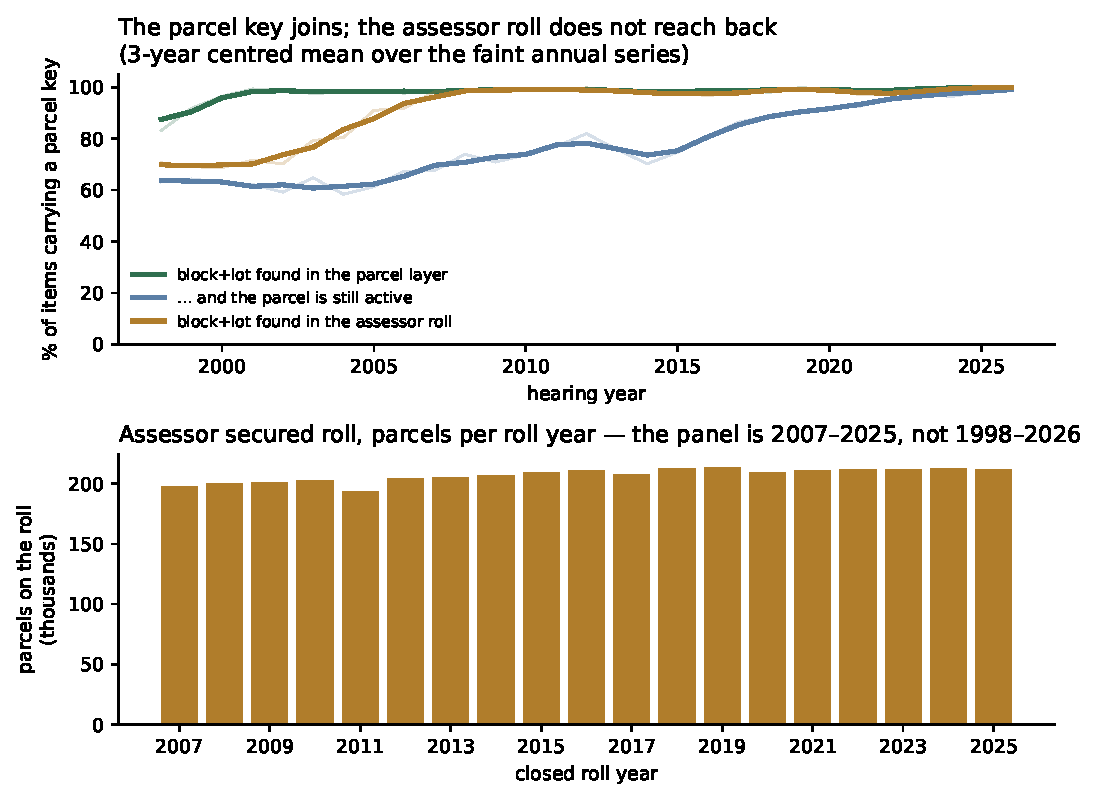
\includegraphics[width=\textwidth]{figures/fig_parcel_riskset.pdf}
\caption{Top: the share of items carrying a parcel key that join the parcel layer, that join
a parcel still active, and that appear on the assessor's roll, by hearing year. Bottom:
parcels on the assessor's secured roll per roll year --- the panel is
\acqAsrFirst--\acqAsrLast, and the bars are flat, so nothing is missing \emph{within} it.}
\label{fig:riskset}
\end{figure}

\subsection{Value: the assessor's secured roll}

\textbf{Assessor Historical Secured Property Tax Rolls} (\texttt{wv5m-vpq2}) is the value
side: \acqAsrRows\ parcel-years over \acqAsrParcels\ distinct parcels, carrying assessed land
value, improvement value, fixtures, use code and definition, property class, year built, lot
area, property area, number of units and stories --- a parcel-year panel in the shape the
hazard needs. Table~\ref{tab:assessor} gives it.

The constraint is the period. \textbf{The roll runs \acqAsrFirst--\acqAsrLast\
(\acqAsrNYears\ years)}, and the corpus runs \acqCorpusSpan. The lower panel of
Figure~\ref{fig:riskset} shows the roll is flat inside its window --- a median of
\acqAsrParcelsPerYear\ parcels a year, every year, with no hole --- so this is a genuine start
date and not the 2018 problem again. Of the \acqAsrSought\ item parcel keys, \acqAsrFound\ appear on the roll at
some point, and \acqAsrJoin\% of items with a parcel key reach it. Of the item parcels that
do appear, \acqAsrBalanced\ appear in every one of the \acqAsrNYears\ years; the rest enter
or leave, so the panel is unbalanced by construction and has to be treated that way.

\paragraph{What this costs.} A parcel-year hazard can be estimated for
\acqAsrFirst--\acqAsrLast. That is within the brief's acceptance range (2005--2026 was asked
for, 1998 was the ideal) but it excludes the first \acqAsrGapYears\ years of the corpus,
which is
precisely the era in which the corpus memo's substitution --- denial falling to zero,
conditioning tripling --- begins. Anything that wants pre-period variation in assessed value
will have to come from somewhere else, and \S\ref{sec:prices} is the only candidate.

\subsection{Zoning, and the one genuinely good surprise}

The brief asked whether any \emph{time-varying} zoning exists, expecting a current snapshot.
It does, and the shape of the publication is the finding. Table~\ref{tab:zoning} is the
inventory.

\begin{itemize}
\item \textbf{\acqZoningParcelYears\ vintages, spanning \acqZoningParcelSpan, are published
\emph{parcel-keyed}}, one row per \texttt{blklot} with the zoning district, the height limit,
the land use and, in the earlier years, unit counts and building square footage. These join to
the item table on the same key as everything else in \S\ref{sec:riskset} and need no spatial
work at all.
\item \textbf{\acqZoningPolygonYears\ more --- the remaining years and the three current
layers (districts, height and bulk, special use) --- are polygon-only.} They are inventoried in
Table~\ref{tab:zoning} with row counts and identifiers and deliberately not cached: turning
them into a parcel panel is a spatial join, which this memo does not do and which should not be
done accidentally.
\item \textbf{One year in the middle of the parcel-keyed run is not published in either
form}, and Table~\ref{tab:zoning} names it.
\end{itemize}

There is also a free current snapshot: \texttt{acdm-wktn} carries \texttt{zoning\_code} and
\texttt{zoning\_district} on every parcel. So current zoning is parcel-keyed,
\acqZoningParcelSpan\ is parcel-keyed, and the years between them are the polygon-only gap in
the middle. That is an odd shape but
it is a far better one than a snapshot, and it means pre-period zoning variation is
available for exactly the era the assessed values are not.

\textbf{Height and bulk is worse.} The historic height-and-bulk series is polygon-only in
every year it is published; there is no parcel-keyed vintage (Table~\ref{tab:negatives}).
Height therefore has to come either from the \acqZoningParcelSpan\ zoning tables'
\texttt{height\_lim} column or from a spatial join.

\textbf{Land use} (\texttt{c5ge-t6pj}) is available as a cross-check on the assessor's use
codes, with one wrinkle: its key is \texttt{mapblklot}, and \acqLandUseMulti\ of its rows
describe a \emph{group} of parcels (\texttt{geography\_type} = \texttt{multiple\_parcels},
with a list of \texttt{mapblklot} values in one cell) rather than a single parcel. That is few
enough to handle as an exception rather than as a design constraint.

\section{Filing dates and the conditional-use-to-permit bridge}
\label{sec:filing}

\subsection{Does the case number join?}

The two Planning Department Records tables --- \texttt{y673-d69b} (Non-Projects,
\acqNonProjRows\ rows) and \texttt{qvu5-m3a2} (Projects, \acqProjRows\ rows) --- are the
department's own
application record. Both identifiers were verified and both are unique on
\texttt{record\_id}. Table~\ref{tab:casejoin} tests the join three ways against all
\acqCases\ distinct cases in the item table.

\begin{itemize}
\item \textbf{Raw string equality: \acqCaseRaw\%.}
\item \textbf{Normalised (upper-case, whitespace stripped): \acqCaseNorm\%.} Normalisation
buys almost nothing here, which is a small vindication of the extraction --- the case numbers
come out clean.
\item \textbf{Suffix-stripped stem: \acqCaseStem\%.} Stripping the letter suffix
(\texttt{2014.0400CUA} $\to$ \texttt{2014.0400}) is what does the work, because it is how a
suffixed case reaches its umbrella project record. \acqCaseAnyN\ of \acqCases\ cases join.
\end{itemize}

Figure~\ref{fig:casejoin} gives it by hearing year, and the residual has one cause.
\textbf{Coverage does not start late; it starts abruptly.} From \acqCaseJoinBreakYear\
onward the annual join rate never falls below \acqCaseJoinLateMin\%. Before that it
collapses, and
Table~\ref{tab:casejoin}'s last block says why: the minutes of that era print the case number
in the two-digit-year form (\texttt{98.426D}), and \textbf{the Planning Department's records
contain no identifier in that format at all --- \acqOldFormatMatched\ of \acqOldFormatCases\
such cases match}. Of the modern-format cases only \acqModernUnmatched\ fail to join. The
residual is a format, not a coverage rate, and no amount of fuzzy matching fixes it: the
records simply do not go back that far under any key.

\begin{figure}[htbp]\centering
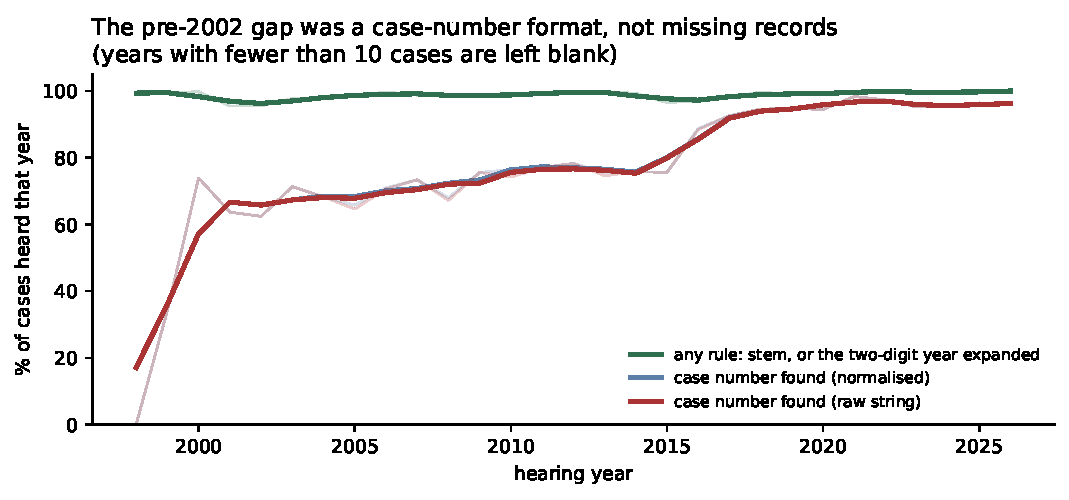
\includegraphics[width=\textwidth]{figures/fig_case_join.pdf}
\caption{Share of cases heard each year whose case number is found in a Planning Department
record, three ways. The early collapse is the two-digit-year case-number format, which the
department's records do not use.}
\label{fig:casejoin}
\end{figure}

\subsection{What \texttt{open\_date} buys: the wait before the hearing}

\texttt{open\_date} is populated on \acqNpOpenDate\% of non-project records
(Table~\ref{tab:recordfields}), so every joined case has one. Collapsing both sides to one row
per case --- earliest open date, earliest hearing --- gives the elapsed time a developer
actually experiences before the Commission first looks at the project.
Table~\ref{tab:filinglag} and Figure~\ref{fig:filinglag} report it.

\begin{itemize}
\item \textbf{Median \acqLagMedian\ days.} 90th percentile \acqLagPninety;
99th \acqLagPninetynine. Coverage \acqLagCoverage\% of all \acqCases\ cases.
\item By request type the ordering is the one the theory wants:
\textbf{variance \acqLagVar\ days, conditional use \acqLagCU, discretionary review
\acqLagDR}. A discretionary review is filed against someone else's pending permit and is
heard quickly; a conditional use is the developer's own application and waits.
\item \acqLagNegative\% of observations are negative --- a record opened after the hearing.
Those are follow-on records, and they are the reason the \emph{earliest} open date of the case
is the one used. They are reported rather than trimmed.
\end{itemize}

\textbf{This is the memo's answer to the delay memo's blind spot.} That memo measures
hearing-to-issuance at a \acqDelayIssueMedian-day median with a \acqDelayIssuePninety-day
90th percentile --- both recomputed here from the artefact that memo wrote, and both
reproduced exactly. The pre-hearing wait is a median of \acqLagMedian\ days with a 90th
percentile of \acqLagPninety: a shorter typical wait and an almost identical tail, and
therefore a markedly larger ratio of tail to centre. A real-options model in which dispersion
is what raises the filing threshold has been ignoring the more dispersed of the two waits, and
starting its clock after the more dispersed one had already run.

\begin{figure}[htbp]\centering
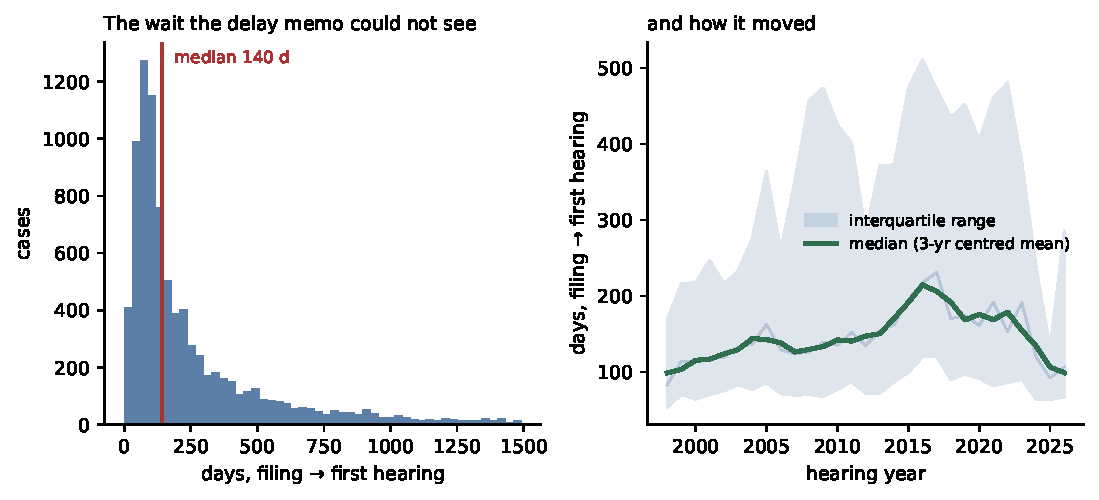
\includegraphics[width=\textwidth]{figures/fig_filing_lag.pdf}
\caption{Left: the distribution of days from filing to first hearing, truncated at
\acqLagTrunc\ days for display;
the median line is computed on the untruncated data. Right: the median by
hearing year with the interquartile range behind it, years with fewer than
\acqMinCasesFig\ cases omitted.}
\label{fig:filinglag}
\end{figure}

\subsection{The bridge, and a correction to the conditions memo}
\label{sec:bridge}

This was the highest-value question in the brief and the answer is yes.

\texttt{building\_permits} is a field on both records tables, populated on
\acqNpBuildingPermits\% of non-project rows and \acqPrBuildingPermits\% of project rows
(Table~\ref{tab:recordfields}). For each item, the
permit numbers were read from the case's own record, from its parent \texttt{PRJ} record where
\texttt{parent\_id} names one, and from any record sharing its stem; each was normalised to
digits exactly as \texttt{analyze\_permits.py} normalises a printed one --- no zero-padding,
because DBI does not pad the serial --- and matched against the cached Building Permits table.
Table~\ref{tab:bridge} is the result.

\begin{itemize}
\item \textbf{Conditional use: \acqBridgeCU\% of \acqBridgeCUTotal\ items reach a permit
present in DBI}, against \acqPrintedCU\% that print a permit number in the minutes. The
route the permit memo had was blind to this part of the docket almost completely; the bridge
is not.
\item Discretionary review reaches \acqBridgeDR\% through the bridge --- \emph{lower} than the
\acqPrintedDR\% that print a number --- so the two routes are complements, not substitutes.
Taking either, \acqEitherDR\% of discretionary reviews reach a permit.
\item \textbf{Across the whole docket, \acqEitherRoute\% of items reach a building permit by
one route or the other}, against \acqBridgeDbiShare\% by the bridge alone and
\acqPrintedAll\% by the printed number alone.
\item Large project authorization (\acqBridgeLpa\%), variance (\acqBridgeVar\%) and
downtown project (\acqBridgeDnt\%) were all effectively unreachable before and are now
reachable. Legislative items (planning code amendment, \acqBridgePca\%) remain unreachable,
correctly --- they are not about a building.
\end{itemize}

\paragraph{Correction.} The conditions memo, \S5.1, concludes:

\begin{quote}\small
``The permit route reaches discretionary review (83.8\% of DR items match a DBI permit) and
essentially nothing else; the conditions route reaches conditional use and essentially nothing
else. Between them they cover most of the docket, but they never cover the same item, so an
analysis that wants both construction outcomes and condition content on one project cannot
have them from these two sources.''
\end{quote}

\noindent
\textbf{That conclusion no longer holds.} \acqBridgeCUN\ conditional-use items --- the exact
population the packet route reaches --- now also reach a building permit in DBI. The
non-overlap was a property of the route, not of the docket: the minutes do not print a permit
number on a conditional use, but the Planning Department records one anyway. Construction
outcomes and condition content \emph{can} be had on the same project, for
\acqBridgeCU\% of conditional uses. \textbf{The conditions memo has been amended
accordingly}: \S5.1 now carries a dated correction paragraph quoting the sentence it
withdraws, and its \S8 item~5 (``the exact complement of the permit route'') has been
narrowed to a claim about what the minutes print rather than about what is knowable.

\subsection{What else the records carry}

Table~\ref{tab:recordfields} inventories the fields the item table does not have, with the
share of rows on which each is actually populated. \texttt{close\_date} (\acqNpCloseDate\%),
\texttt{record\_status} (\acqNpRecordStatus\%), \texttt{applicant} (\acqNpApplicant\%),
\texttt{assigned\_to\_planner} (\acqNpPlanner\%) and \texttt{applicant\_org}
(\acqNpApplicantOrg\%) are all substantially populated and all are new information. Two are
not what their names suggest: \texttt{project\_decision} is populated on \acqPrDecision\% of
project rows, so the department's own decision field is not a substitute for the extraction,
and \texttt{inclusionary} is a flag on \acqPrInclFlag\%.

\section{Project scale}
\label{sec:scale}

Table~\ref{tab:scale} is the answer, and it contains the memo's clearest instance of the
difference between a field existing and a field carrying information.

\textbf{The Projects table is the spine.} Its \texttt{number\_of\_units\_prop} reaches
\acqCuUnits\% of conditional-use items through the case-number stem, over a date range that
starts long before any purpose-built pipeline dataset. But the field is never null and is
\emph{zero} on most rows: \textbf{it is non-zero on only \acqCuUnitsNZ\% of conditional-use
items}. Reporting the first number alone would be reporting the documentation. The right
statement is that a unit count is \emph{attached} to the great majority of conditional uses
and is \emph{informative} on well under a third of them --- which is consistent with the
docket, most of which is not residential construction, but which caps what a revenue measure
built on it can do.

The purpose-built datasets are weaker than the brief hoped:

\begin{itemize}
\item \textbf{SF Development Pipeline} (\texttt{6jgi-cpb4}) does carry a planning case number
--- \texttt{case\_no} --- which is what the brief flagged as a potential P0 find. It is the
\texttt{PRJ} umbrella number, so it reaches the item table only through the stem, and it is a
\textbf{current snapshot}: \acqPipelineRows\ rows, the projects in the pipeline now. It
reaches
\acqCuPipeline\% of conditional-use items. It is a good source for scale on live projects and
not a panel.
\item \textbf{Housing Production 2005--present} (\texttt{xdht-4php}) carries
\texttt{ppts\_project\_id} in the old \texttt{YYYY.NNNN} form, which joins to the item table's
stem, and \texttt{blocklot}. It reaches \acqCuHousingProd\% of conditional-use items by
parcel. It is completions, so it observes only projects that were built.
\item \textbf{MOHCD Affordable Housing Pipeline} (\texttt{aaxw-2cb8}) carries
\texttt{planning\_case\_number} explicitly and is \acqMohcdRows\ rows. It reaches
\acqCuMohcd\% of
conditional-use items. It is the right source for the affordability channel and it is small.
\item \textbf{Dwelling Unit Completion Counts} (\texttt{j67f-aayr}) is keyed on the building
permit number, so it is reachable only through \S\ref{sec:bridge}'s bridge --- which is now a
reason it is reachable at all.
\end{itemize}

\textbf{And none of it reaches the early docket well.} Every purpose-built scale dataset
begins in \acqScaleEarliest\ or later, and the consequence is measurable rather than
rhetorical: a non-zero unit count reaches \acqCuUnitsNZearly\% of conditional uses heard
before \acqScaleEarliest\ against \acqCuUnitsNZlate\% of those heard after.

\section{Prices and rents}
\label{sec:prices}

Table~\ref{tab:prices} is the fallback chain. The top of it is the finding.

\paragraph{CoreLogic / Cotality: the pull happened, and the extract is here.} The brief
asked whether the pull went through before Stanford access lapsed. It did, and the files are
under the data root: \texttt{demand/} holds \acqDemandFiles\ files and \acqDemandGB\,GB,
including both the raw Cotality extracts and the cleaned parquet
\texttt{demand\_estimation/corelogic.py} built from them.

\textbf{An earlier pass of this memo reported the whole \texttt{demand/} subtree as absent.
It was wrong, and the reason is worth recording because it will recur.} Dropbox's macOS file
provider keeps files \emph{online-only}: the directory entry reports the full size while the
file occupies zero blocks, and a directory that has never been materialised does not appear in
a listing at all. \texttt{find} and \texttt{ls} both said nothing was there.
\texttt{acquire\_external\_data.py sync} is now the check --- it reports nominal bytes
against bytes on disk and materialises what is dehydrated --- and running it turned up
\acqDemandGB\,GB across \acqDemandFiles\ files, of which several gigabytes were
placeholders. \textbf{The lesson is the one the repo already knows in another form: when the
machine and the record disagree, check the source before believing the machine.}

\paragraph{What it is, and that it joins at the parcel.} Table~\ref{tab:prices} and
Figure~\ref{fig:corelogic} report it. The extract holds \acqClRows\ San Francisco
transactions, of which \acqClPriced\ are arms-length with a price and \acqClResidential\
are residential, over \acqClParcels\ distinct parcels.

The join is the find. Cotality prints San Francisco's APN as \texttt{0836 003} --- block and
lot, in the same four-plus-three form DataSF uses --- so stripping the separator yields
\texttt{blklot} directly. \textbf{\acqClKeyed\% of San Francisco transactions carry a
usable parcel key}, and the price therefore joins to the item table on exactly the key the
risk set of \S\ref{sec:riskset} is built on. This is a parcel-level price, not a
market-level index, and it is the difference between having $\Pi(s)$ and having a proxy
for it.

What that buys, measured rather than asserted:

\begin{itemize}
\item \textbf{\acqClItemKeysTraded\ of the \acqClItemKeys\ distinct parcels the item
table touches (\acqClItemKeysTradedPct\%) have at least one arms-length sale.}
\item \textbf{\acqClItemsEverPct\% of items with a parcel key} sit on a parcel that has
traded at some point --- \acqClItemsEver\ items.
\item \textbf{\acqClItemsNearPct\% sit on a parcel that traded within
\acqClWindowYears\ years of the hearing} (\acqClItemsNear\ items). That is the number
that matters for a filing threshold: it is the share of decisions for which a
\emph{contemporaneous} market price on the actual parcel is observable, rather than a
neighbourhood average.
\end{itemize}

The right panel of Figure~\ref{fig:corelogic} shows the first of those rising from roughly
half to three quarters over the period, as more of the housing stock turns over at least once
inside the window the extract covers, while the contemporaneous-trade share sits flat near a
quarter. The flatness is the honest read: turnover, not data coverage, is what caps it.

\begin{figure}[htbp]\centering
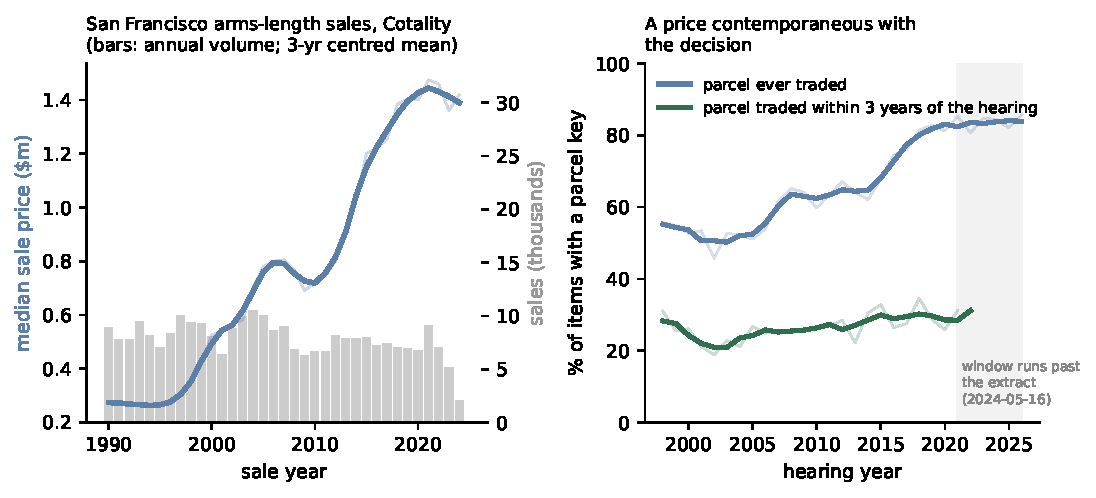
\includegraphics[width=\textwidth]{figures/fig_corelogic.pdf}
\caption{Left: median arms-length sale price in San Francisco with annual volume behind it,
from the year the extract becomes dense. Right: the share of items carrying a parcel key whose
parcel has ever traded, and whose parcel traded within \acqClWindowYears\ years of the
hearing. The shaded band is the hearing years whose forward window runs past the end of the
extract; the contemporaneous series is not drawn there, because a fall would be an artefact of
where the file stops.}
\label{fig:corelogic}
\end{figure}

\paragraph{Where it stops.} The extract ends \acqClMaxDate, two years short of the corpus,
and the series is only dense from \acqClDenseFirst\ (a handful of deeds carry placeholder
dates back to \acqClFirst). The last three hearing years therefore cannot have a
\acqClWindowYears-year forward window and are drawn as a gap in Figure~\ref{fig:corelogic}
rather than as a decline --- the same rule the corpus memo applies to 2018.

\paragraph{CoStar} is an access question and is reported as one. Nothing was attempted and
nothing was scraped.

\paragraph{What is cached instead.} Zillow's research files, filtered to San Francisco County
and stored with the national row counts recorded so the filter is auditable:
\textbf{ZHVI on \acqZhviZips\ ZIP codes, \acqZhviFirst\ to \acqZhviLast}, and
\textbf{ZORI on \acqZoriZips\ ZIP codes, \acqZoriFirst\ to \acqZoriLast}. These are
market-level indices; the item table has no ZIP, so using them means going parcel $\to$
address $\to$ ZIP, or falling back to the supervisor district and analysis neighbourhood the
parcel layer already carries. They are a price \emph{environment}, not a project price.

\paragraph{The fallback.} Assessed land and improvement value from \S\ref{sec:riskset},
parcel-year, \acqAsrFirst--\acqAsrLast, universal within that window. It is a weak price:
Proposition~13 makes assessed value a function of how long the current owner has held the
parcel rather than of what the parcel is worth. It is worth having with that caveat stated in
every table it appears in, and it is not a substitute for a transaction price.

\section{Fee and exaction schedules}
\label{sec:fees}

The conditions memo finds that most staff-imposed conditions are obligation-imposing rather
than project-changing, and that the largest recurring headings --- Transportation Sustainability Fee, inclusionary,
impact fees --- have posted dollar schedules. This section converts those headings into
dollars.

\paragraph{The document.} The \textbf{San Francisco Citywide Development Impact Fee Register}
is a multi-page landscape schedule, republished each January, giving for every fee: the city
area subject to it, the ordinance reference, the uses it applies to, the rate, the threshold,
the controlling entity, the unit, and the effective date. It is exactly the object the brief
asked for.

\paragraph{The problem, and the route around it.} The register is republished at \emph{one
URL}, so the department's site only ever holds the current year. \acqFeeRegisters\ dated
copies were assembled --- \acqFeeFirst\ through \acqFeeLast\ --- from the Wayback Machine's
snapshots of that URL and from the year-stamped URLs the department left behind.
\textbf{No snapshot exists before \acqFeeEarliestSnapshot}, under that URL or any other
tried, so the
fee panel starts at \acqFeeFirst\ (Table~\ref{tab:negatives}).

\paragraph{The parse.} Table~\ref{tab:fees} reports what came out of each register:
\acqFeeRates\ dated rate observations in total, keyed to the Planning Code (or State
Education Code) section of the register row they sit in, and to the land-use or size band the
register prints on the same line. The section is the key because it is the only column that
survives PDF text extraction intact; the fee \emph{name} wraps across several lines and the
columns interleave. Effective dates are read from the register's own cover line, not inferred
from when the file was retrieved.

Table~\ref{tab:feerates} is the result: \textbf{a rate keyed by year, by fee and, where the
register labels it, by land use}. The Transportation Sustainability Fee for residential
projects over 99 units runs \$\acqTsfNinetyNineFirst\ per gross square foot in \acqFeeFirst\
to \$\acqTsfNinetyNineLast\ in \acqFeeLast; the inclusionary fee under \S415 runs
\$\acqInclusionaryFirst\ to \$\acqInclusionaryLast\ per square foot of residential gross floor
area. A named condition heading in a Commission motion can now be priced.

\paragraph{What is not here.} The register's \emph{district} dimension is a free-text column
(``Eastern Neighborhoods Mixed Use Districts: RED, RED-MX, SPD, MUG\ldots'') and is not parsed
into a key. Neighborhood-Specific Impact Fee Areas (\texttt{ntc3-dd64}, \acqFeeAreaRows\
rows) is cached and
is the geographic side of that, but joining a fee area to a parcel is a spatial join and is
not done here. The inclusionary \emph{requirement percentages} under \S415 --- as distinct
from the in-lieu fee --- and their amendment history are legislative and are not in the
register; that remains open.

\section{Established, and not established}

\textbf{Established.}
\begin{enumerate}
\item A parcel-year risk set can be built. \texttt{acdm-wktn} is unique on \texttt{blklot} and
\acqParcelJoin\% of items carrying a parcel key join to it; the residual is
\acqParcelNoLot\ block-matched lot failures and \acqParcelNoBlock\ unmatched blocks, not a
formatting problem.
\item The value side of that risk set is \acqAsrFirst--\acqAsrLast\ and no earlier.
\acqAsrRows\ parcel-years, flat across the window, \acqAsrJoin\% of keyed items reached.
\item Zoning is time-varying and parcel-keyed for \acqZoningParcelYears\ vintages spanning
\acqZoningParcelSpan, and polygon-only for \acqZoningPolygonYears\ more.
\item The case number joins the Planning Department's records on \acqCaseAny\% of
\acqCases\ cases, via the suffix-stripped stem, and never below \acqCaseJoinLateMin\% in any
year from \acqCaseJoinBreakYear\ on. The earlier residual is entirely the two-digit-year
case-number format.
\item Filing to first hearing is measurable on \acqLagCoverage\% of cases: median
\acqLagMedian\ days, 90th percentile \acqLagPninety, 99th \acqLagPninetynine.
\item The \texttt{building\_permits} bridge reaches \acqBridgeCU\% of conditional-use items
through to a permit present in DBI, and \acqEitherRoute\% of the docket reaches a permit by
some route. The conditions memo's non-overlap claim (\S5.1) is overturned.
\item A unit count is attached to \acqCuUnits\% of conditional-use items and is non-zero on
\acqCuUnitsNZ\%.
\item The CoreLogic extract is present, and it is a \emph{parcel-level} price:
\acqClPriced\ arms-length San Francisco sales over \acqClParcels\ parcels, keyed on
\texttt{blklot} on \acqClKeyed\% of transactions. \acqClItemsEverPct\% of items with a
parcel key sit on a parcel that has traded, \acqClItemsNearPct\% on one that traded within
\acqClWindowYears\ years of the hearing.
\item An annual dollar fee schedule exists for \acqFeeFirst--\acqFeeLast, keyed by Planning
Code section and land-use band, \acqFeeRates\ rate observations.
\end{enumerate}

\textbf{Not established.}
\begin{enumerate}
\item Whether the \acqParcelNoLot\ block-matched, lot-unmatched items are extraction errors or
lots the recorder never carried. The block matched, so both are live; a hand pass on a sample
would settle it and has not been done.
\item Whether a case's \emph{earliest} \texttt{open\_date} is the filing date a developer
would recognise. A case can have several records opened under one stem --- environmental,
preliminary project assessment, the entitlement itself --- and the earliest is the earliest
\emph{administrative} act, which may pre-date the application the hearing is about. The
\acqLagPninetynine-day 99th percentile is the visible symptom.
\item Whether the permit a conditional use reaches through the bridge is the permit the
hearing was \emph{about}. The bridge returns every permit the department associates with the
project; no adjudication of which one is the entitlement's permit has been done, and the
permit memo's parcel-window-type rule is the obvious tool for it.
\item Whether \texttt{number\_of\_units\_prop} means the same thing across the Projects
table's full span. It is zero on most rows and the zero is not distinguishable from an
unfilled field.
\item Anything about fee levels before \acqFeeFirst. The register panel starts there and the
earlier schedules are not on the site or in the archive under any URL tried.
\item Whether a sale near the hearing is a sale \emph{caused} by it, or how to treat the
parcels that never trade. \acqClItemsNearPct\% of keyed items have a contemporaneous price;
the complement is not missing at random --- a parcel that has not changed hands in decades is
a different kind of parcel --- and nothing here corrects for that.
\item Anything causal. Every number in this memo is a coverage rate or a descriptive
distribution.
\end{enumerate}

\section{Limitations}

\paragraph{Coverage rates resting on a small denominator.} The MOHCD pipeline is
\acqMohcdRows\ rows and
reaches \acqCuMohcd\% of conditional-use items --- that is a handful of items, and a rate
computed on it should not be reported to one decimal place anywhere but the table it comes
from. The Development Pipeline's \acqCuPipeline\% rests on \acqPipelineRows\ rows. The
request-type breakdown in Table~\ref{tab:bridge} suppresses types with fewer than
\acqMinItemsBridge\ items, and Table~\ref{tab:filinglag} suppresses groups with fewer than
\acqMinCasesFig\ cases with a lag.

\paragraph{Current snapshots that are not panels.} The Development Pipeline is the projects in
the pipeline \emph{now}; a project entitled a decade ago and long since built is not in it.
The
current zoning, height-and-bulk and special-use layers are snapshots. \texttt{acdm-wktn}'s
\texttt{zoning\_code} is current zoning attached to every parcel including retired ones, which
is a snapshot wearing a panel's clothes and must not be used as the zoning \emph{at} the time
of an early hearing --- that is what the \acqZoningParcelSpan\ vintages are for. San Francisco Land Use is
one \texttt{data\_as\_of} date.

\paragraph{Periods that do not line up.} The corpus is \acqCorpusSpan. Assessed values are
\acqAsrFirst--\acqAsrLast. Parcel-keyed zoning is \acqZoningParcelSpan. Fee rates are
\acqFeeFirst--\acqFeeLast. Transaction prices are \acqClDenseFirst--\acqClLast\ and stop
at \acqClMaxDate. \textbf{No single window has all of them}, and a specification
wanting both an assessed value and the zoning in force is confined to the overlap of the
second and third unless the polygon zoning years are joined spatially.

\paragraph{Access questions left open.} CoStar (BU Questrom holdings, unchecked by design).
The \S415 inclusionary requirement percentages and their amendment history. Fee registers
before \acqFeeFirst. CoreLogic is \emph{not} on this list any more --- the extract is on
disk --- but the licence is Stanford's and lapsed, so the file cannot be refreshed past
\acqClMaxDate\ without new access. Treat what is cached as frozen.

\paragraph{Source quirks worth carrying.} Dwelling Unit Completion Counts contains a
\texttt{date\_issued} in \acqUcMaxYear, marked \emph{(sic)} in Tables~\ref{tab:inventory}
and~\ref{tab:scale}; it is a typo in the source, not the end of the file's coverage. The MOHCD
pipeline's dates run to \acqMohcdMaxYear\ because they are estimated construction completions,
which is
correct. \acqNonUniqueSources\ of the \acqSourcesCached\ cached sources are not unique on
their intended key and are marked so in Table~\ref{tab:inventory}. The Planning Department's non-project table has an
\texttt{open\_date} in \acqNpMinYear, which is real in the sense that the row says so and has
not been audited.

\paragraph{One measurement not attempted.} The brief asks for a sample of non-joining parcel
keys with the reason. Table~\ref{tab:parceljoin} gives the reasons as a partition ---
retired-only, block-matched-lot-unmatched, no-such-block --- which is the aggregate version of
that, and the sample of individual keys is left for the hand pass in ``Not established''
item~1.

\section{Reproducing this}

\texttt{code/commission\_minutes\_processing/acquire\_external\_data.py} runs in three stages,
each cached so no network stage repeats by accident:

\begin{verbatim}
python acquire_external_data.py sync             # materialise online-only files
python acquire_external_data.py probe            # resolve every identifier, live
python acquire_external_data.py fetch            # download and cache each source
python acquire_external_data.py fetch --refresh  # re-download everything
python acquire_external_data.py fetch --only assessor   # or one source
python acquire_external_data.py report           # joins, figures, tables, README
\end{verbatim}

\texttt{sync} materialises every online-only file under
\texttt{\$MFHR\_DATA\_ROOT/demand/} and prints nominal bytes against bytes on disk.
Run it first: it is the difference between a subtree that is missing and one that Dropbox has
simply not downloaded, and this memo got that wrong once.

\texttt{probe} writes \texttt{\$MFHR\_DATA\_ROOT/external/\_acquisition/probe.json} --- the
resolved identifier, row count, column list and update time for every dataset, the catalogue
searches that produced them, and an HTTP check on every non-Socrata file. \texttt{fetch}
writes one directory per source under \texttt{\$MFHR\_DATA\_ROOT/external/}
(\texttt{parcels}, \texttt{assessor}, \texttt{zoning}, \texttt{planning\_records},
\texttt{pipeline}, \texttt{prices}, \texttt{fees}) and skips anything already on disk.
\texttt{fetch -{}-only corelogic} is the exception that downloads nothing: it slices the
licensed Cotality extract already under \texttt{demand/} down to San Francisco, attaches the
parcel key, and caches the result, so \texttt{report} does not re-read two gigabytes.
\texttt{report} regenerates the three figures, \texttt{tables/acquisition\_tables.tex},
\texttt{tables/acquisition\_macros.tex}, and \texttt{external/README.md}, which records per
source the resolved identifier, retrieval date and row count so a later run can tell whether
the cache is stale.

The item table is the same extraction the other memos read
(\texttt{\$MFHR\_DATA\_ROOT/}\allowbreak\texttt{extraction/corpus\_v2\_g3/clean/*.jsonl}),
and the permit
normalisation and the printed-permit parser are imported from
\texttt{analyze\_permits.py} rather than re-implemented, so the two memos cannot report
different numbers for the same question.

\textbf{No number in this memo is hand-placed}, and here that is literal rather than
conventional. Every measurement in the prose is a \texttt{\textbackslash newcommand} defined
in \texttt{tables/acquisition\_macros.tex}, written by \texttt{report}; the tables are
\texttt{tables/acquisition\_tables.tex}, written by the same function; both are
\texttt{\textbackslash input} at the top of the \texttt{.tex}. Changing a figure in this
document means changing the script.

The only numerals typed into the \texttt{.tex} are: section and item cross-references;
identifiers and dataset names (\texttt{2014.0400CUA}, \texttt{98.426D}, Housing
Production 2005--present); the register's own printed land-use bands
(``over 99 units''); named prior facts (Proposition~13, the 2018 hole in the meeting corpus);
the brief's own $\geq$95\% acceptance criterion; and three figures quoted from sibling memos,
each
attributed where it appears --- the corpus memo's 8{,}295 distinct parcels, the permit memo's
145{,}795 duplicate \texttt{permit\_number} rows, and the 83.8\% inside the block quotation
from the conditions memo. The delay memo's hearing-to-issuance median is \emph{not} in that
list: \texttt{report} recomputes it from \texttt{permit\_matches.csv} and it appears here as
\texttt{\textbackslash acqDelayIssueMedian}, which is one way of checking that this memo and
that one still agree.

\end{document}
